\documentclass[tikz]{standalone}
\usepackage{pgfplots}
\pgfplotsset{compat=1.15}
\usepackage{mathrsfs}
\usetikzlibrary{arrows,calc}
\usepackage{tkz-euclide}
\pagestyle{empty}

\definecolor{AngleClr}{rgb}{0,0.39215686274509803,0}
\definecolor{ShapeClr}{rgb}{0.6,0.2,0}

\begin{document}

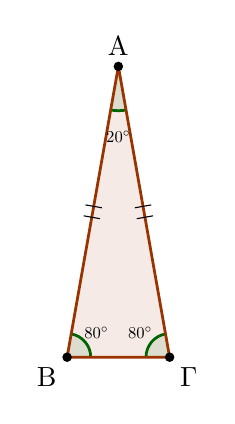
\begin{tikzpicture}[scale=.75]
\tkzSetUpLine[line width=1pt,color=black]
\tkzSetUpPoint[fill=black]

\tkzDefPoints{-0.868/0/B,0/4.924/A,0.868/0/C}

\tkzFillPolygon[fill=ShapeClr,fill opacity=0.1](A,B,C)
\tkzFillAngles[fill=AngleClr,size=.4,fill opacity=0.1](C,B,A A,C,B)
\tkzMarkAngles[line width=1pt,size=.4,color=AngleClr](C,B,A A,C,B)

\tkzFillAngles[fill=AngleClr,size=.75,fill opacity=0.1](B,A,C)
\tkzMarkAngles[line width=1pt,size=.75,color=AngleClr](B,A,C)

\tkzDrawPolygon[color=ShapeClr](A,B,C)
\tkzDrawPoints[size=3](A,B,C)
\tkzLabelPoint[above](A){$\rm A$}
\tkzLabelPoint[below left](B){$\rm B$}
\tkzLabelPoint[below right](C){$\rm \Gamma$}

\tkzLabelAngle[pos=0.65](C,B,A){\scalebox{0.6}{$80^\circ$} }
\tkzLabelAngle[pos=0.65](A,C,B){\scalebox{0.6}{$80^\circ$} }
\tkzLabelAngle[pos=1.2](B,A,C){\scalebox{0.6}{$20^\circ$} }

\tkzMarkSegments[mark=||,size=3](A,B C,A)


\end{tikzpicture}

\end{document}
